\section{Experiments}
\label{sec:experiments}
\textbf{Details on implementation, datasets, and computational cost are provided in the Supplementary Materials}.

\subsection{Tasks and Datasets}
We conduct four core evaluations to comprehensively assess MMRL's performance: base-to-novel generalization, cross-dataset evaluation, domain generalization, and few-shot learning. Except for few-shot learning, all experiments utilize a 16-shot setting, \ie., only 16 training examples per category.

\noindent \textbf{Base-to-Novel Generalization:} 
In this evaluation, dataset classes are equally divided into base and novel classes. The model is trained exclusively on base classes and tested on both base and novel classes, allowing us to examine its transfer learning effectiveness on base classes as well as its ability to retain the inherent generalization or zero-shot capabilities of pre-trained VLMs for novel classes. We conduct this evaluation across 11 diverse image classification datasets: ImageNet \cite{imagenet}, Caltech101 \cite{caltech101}, OxfordPets \cite{oxford_pets}, StanfordCars \cite{stanford_cars}, Flowers102 \cite{flowers102}, Food101 \cite{food101}, FGVCAircraft \cite{fgvc_aircraft}, SUN397 \cite{sun397}, UCF101 \cite{ucf101}, DTD \cite{dtd}, and EuroSAT \cite{eurosat}.

\noindent \textbf{Cross-Dataset Evaluation:} This evaluation measures the model’s transferability to new, unseen datasets. Following CoCoOp \cite{cocoop}, we train the model on all 1000 ImageNet classes in a few-shot setting and then directly apply it, without further fine-tuning, to other datasets to assess its cross-dataset generalization. We employ the same datasets as in the base-to-novel generalization task.

\noindent \textbf{Domain Generalization:} In this setting, we assess the resilience of the ImageNet-trained model to domain shifts and its generalization to out-of-distribution data. Specifically, we use ImageNet as the training dataset and evaluate on four variants—ImageNetV2 \cite{imagenetv2}, ImageNet-Sketch \cite{imagenet_sketch}, ImageNet-A \cite{imagenet_a}, and ImageNet-R \cite{imagenet_r}—each introducing different types of domain variation.

\noindent \textbf{Few-Shot Learning:} This evaluation examines the model's transfer learning capability in limited-data scenarios, independent of its generalization performance. The model is trained on subsets of the training data with 1, 2, 4, 8, and 16 examples (shots) per class and subsequently evaluated on the full test sets. 



\begin{table*}[t]
\centering
\setlength{\abovecaptionskip}{0.15cm}  
\caption{Comparison of MMRL with previous state-of-the-art methods on cross-dataset evaluation across 10 datasets.}
\label{cross_dataset}
\resizebox{0.9\textwidth}{!}{
    \footnotesize
    \begin{tabular}{@{}rc|ccccccccccc@{}}
    \toprule
     &
      Source &
      \multicolumn{11}{c}{Target} \\ \cmidrule(l){2-13} 
     &
      \rotatebox{60}{ImageNet} &
      \rotatebox{60}{Average} &
      \rotatebox{60}{Caltech101} &
      \rotatebox{60}{OxfordPets} &
      \rotatebox{60}{StanfordCars} &
      \rotatebox{60}{Flowers101} &
      \rotatebox{60}{Food101} &
      \rotatebox{60}{FGVCAircraft} &
      \rotatebox{60}{SUN397} &
      \rotatebox{60}{DTD} &
      \rotatebox{60}{EuroSAT} &
      \rotatebox{60}{UCF101} \\ \cmidrule(l){2-13} 
    $\text{CoOp}_{\text{ (IJCV2022)}}$ &
      71.51 &
      63.88 &
      93.70 &
      89.14 &
      64.51 &
      68.71 &
      85.30 &
      18.47 &
      64.15 &
      41.92 &
      46.39 &
      66.55 \\
    $\text{CoOpOp}_{\text{ (CVPR2022)}}$ &
      71.02 &
      65.74 &
      94.43 &
      90.14 &
      65.32 &
      71.88 &
      86.06 &
      22.94 &
      67.36 &
      45.73 &
      45.37 &
      68.21 \\
    $\text{MaPLe}_{\text{ (CVPR2023)}}$ &
      70.72 &
      66.30 &
      93.53 &
      90.49 &
      65.57 &
      72.23 &
      86.20 &
      24.74 &
      67.01 &
      46.49 &
      48.06 &
      68.69 \\
    $\text{PromptSRC}_{\text{ (ICCV2023)}}$ &
      71.27 &
      65.81 &
      93.60 &
      90.25 &
      65.70 &
      70.25 &
      86.15 &
      23.90 &
      67.10 &
      \textbf{46.87} &
      45.50 &
      \textbf{68.75} \\
    $\text{TCP}_{\text{ (CVPR2024)}}$ &
      71.40 &
      66.29 &
      93.97 &
      91.25 &
      64.69 &
      71.21 &
      \textbf{86.69} &
      23.45 &
      67.15 &
      44.35 &
      51.45 &
      68.73 \\
    $\text{MMA}_{\text{ (CVPR2024)}}$ &
      71.00 &
      66.61 &
      93.80 &
      90.30 &
      \textbf{66.13} &
      72.07 &
      86.12 &
      25.33 &
      \textbf{68.17} &
      46.57 &
      49.24 &
      68.32 \\ \midrule
    $\text{MMRL}_{\text{ (Ours)}}$ &
      \textbf{72.03} &
      \textbf{67.25} &
      \textbf{94.67} &
      \textbf{91.43} &
      66.10 &
      \textbf{72.77} &
      86.40 &
      \textbf{26.30} &
      67.57 &
      45.90 &
      \textbf{53.10} &
      68.27 \\ \bottomrule
    \end{tabular}
    }
\vspace{-0.3cm}
\end{table*}




%-------------------------------------------------------------------------
\begin{figure*}[t]
\centering
\setlength{\belowcaptionskip}{-0.39cm}  
  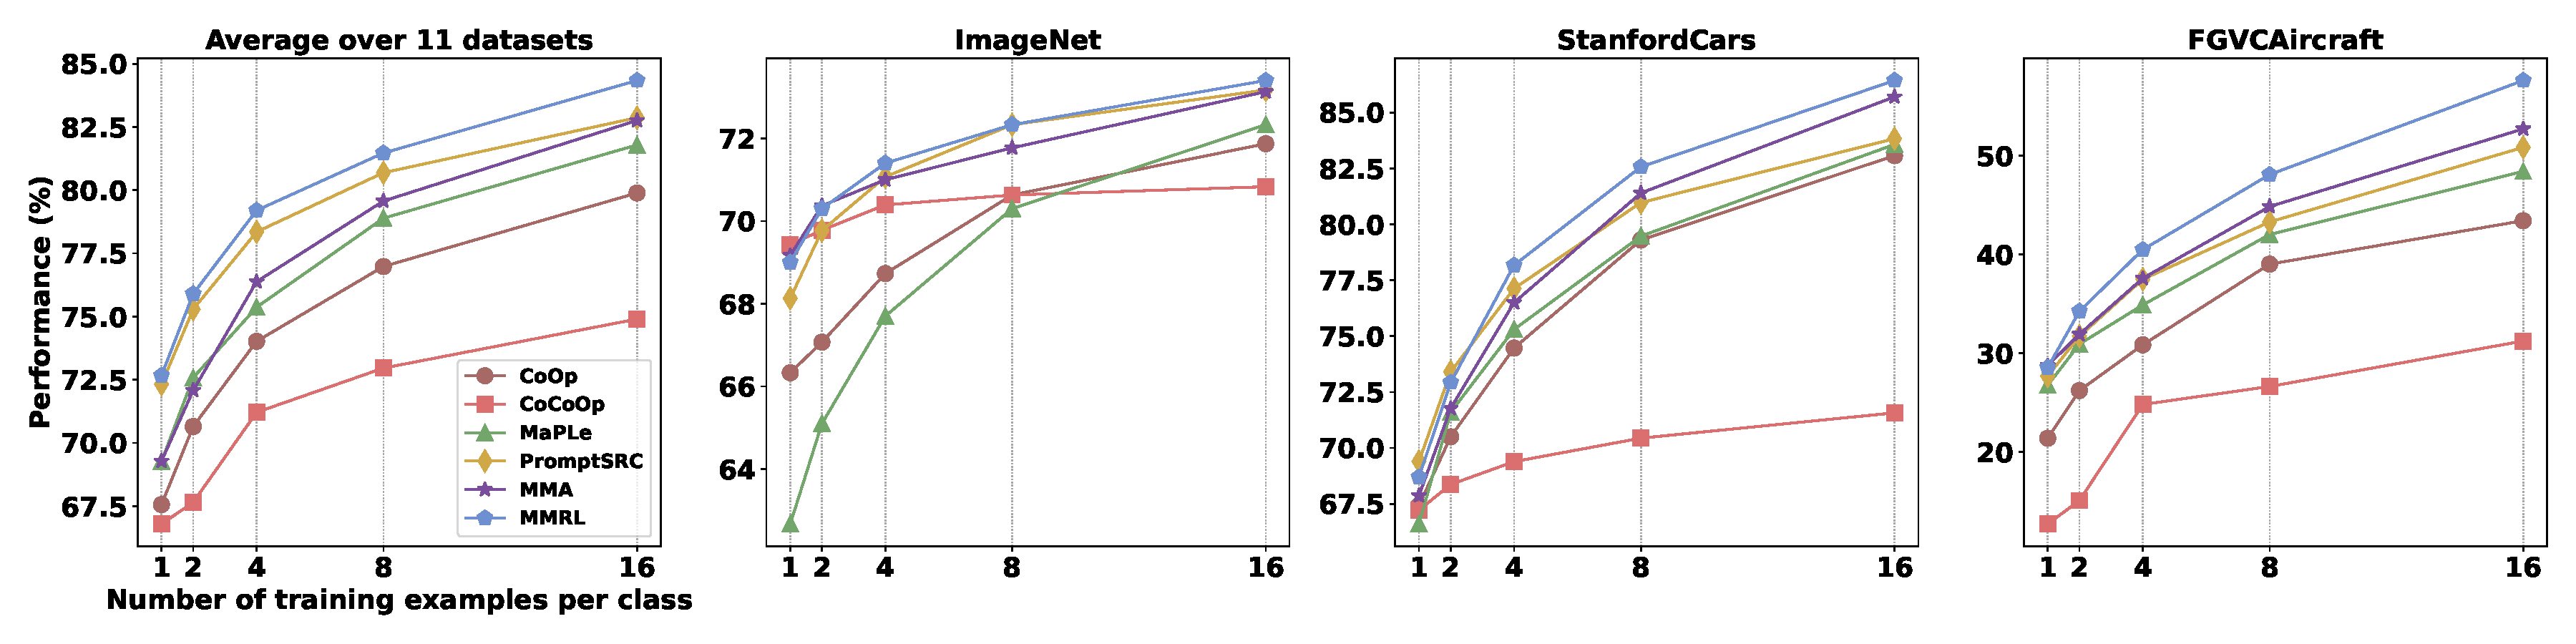
\includegraphics[width=0.9\linewidth]{fig/few_shot.pdf}
  \vspace{-0.3cm}
  \caption{Comparison of MMRL with previous state-of-the-art methods on few-shot learning across 11 datasets. Detailed results on all 11 datasets are provided in the \textbf{Supplementary Material}.}
  \label{few_shot_figure}
\end{figure*}
%-------------------------------------------------------------------------



\subsection{Base-to-Novel Generalization}

In this experiment, we compare MMRL with several models, including the zero-shot baseline CLIP and leading prompt learning approaches: CoOp \cite{coop}, CoCoOp \cite{cocoop}, ProDA \cite{proda}, KgCoOp \cite{kgcoop}, MaPLe \cite{maple}, PromptSRC \cite{promptsrc}, ProVP \cite{provp}, MetaPrompt \cite{metaprompt}, TCP \cite{tcp} and the multimodal adapter-style model MMA \cite{mma}. 

\cref{base_to_novel} provides detailed results for \textbf{Base} and \textbf{Novel} classes across 11 datasets, along with the balanced harmonic mean (\textbf{HM}) of their accuracies. Key findings include:

\noindent \textbf{New SOTA Performance:} Based on the average results across 11 datasets, MMRL achieves gains of 2.48\%, 0.36\%, and 1.33\% in Base, Novel, and HM metrics, respectively, surpassing the previous best-performing model, MMA, and establishing a new state-of-the-art.

\noindent \textbf{Strong Generalizability with Enhanced Transfer Learning:} Notably, MMRL enhances generalizability while significantly boosting base accuracy, effectively improving transfer learning capabilities across downstream datasets such as ImageNet, StanfordCars, and SUN397. Although MMRL may not consistently achieve the highest novel accuracy on some datasets (e.g., UCF101, EuroSAT, DTD, and FGVCAircraft), it substantially outperforms other methods in the base category. For instance, on FGVCAircraft, MMRL’s novel accuracy trails PromptSRC by 0.84\%, yet it achieves a significant 3.57\% gain in base accuracy. Similarly, on EuroSAT, MMRL underperforms MMA by 2.17\% in the novel category but outperforms it by 10.14\% in the base category!


\begin{table}[t]
\centering
\setlength{\abovecaptionskip}{0.15cm}  
\caption{Comparison of MMRL with previous state-of-the-art methods on domain generalization across 4 datasets.}
\label{domain_generalization}
\resizebox{0.45\textwidth}{!}{
    \footnotesize
    \begin{tabular}{@{}rc|cccc@{}}
    \toprule
                                         & Source   & \multicolumn{4}{c}{Target}    \\ \cmidrule(l){2-6} 
                                         & ImageNet & -V2   & -S    & -A    & -R    \\ \cmidrule(l){2-6} 
    $\text{CLIP}_{\text{ (ICML2021)}}$   & 66.73    & 60.83 & 46.15 & 47.77 & 73.96 \\
    $\text{CoOp}_{\text{ (IJCV2022)}}$   & 71.51    & 64.20 & 47.99 & 49.71 & 75.21 \\
    $\text{CoOpOp}_{\text{ (CVPR2022)}}$ & 71.02    & 64.07 & 48.75 & 50.63 & 76.18 \\
    $\text{MaPLe}_{\text{ (CVPR2023)}}$  & 70.72    & 64.07 & 49.15 & 50.90 & 76.98 \\
    $\text{PromptSRC}_{\text{ (ICCV2023)}}$ & 71.27          & 64.35          & \textbf{49.55} & 50.90          & \textbf{77.80} \\
    $\text{MMA}_{\text{ (CVPR2024)}}$    & 71.00    & 64.33 & 49.13 & 51.12 & 77.32 \\ \midrule
    $\text{MMRL}_{\text{ (Ours)}}$          & \textbf{72.03} & \textbf{64.47} & 49.17          & \textbf{51.20} & 77.53 \\ \bottomrule
    \end{tabular}
    }
\vspace{-0.4cm}
\end{table}

\subsection{Cross-Dataset Evaluation}
As illustrated in \cref{cross_dataset}, MMRL achieves a 1.03\% accuracy improvement over the previous state-of-the-art method, MMA, on ImageNet. Beyond this, MMRL consistently exhibits superior performance across various target datasets, achieving the highest average accuracy, which underscores its strong cross-dataset generalization capability.

\subsection{Domain Generalization}
As summarized in \cref{domain_generalization}, MMRL attains top performance on 2 out of the 4 domain-shifted datasets, showcasing its robust generalization capability across diverse domains.


\subsection{Few-Shot Learning}
As shown in \cref{few_shot_figure}, MMRL achieves the best average performance across 11 datasets under all shot settings, with performance margins increasing as the shot number rises. This trend confirms MMRL’s strong transfer learning capability, even in data-scarce scenarios.


%-------------------------------------------------------------------------
\begin{figure}[tb]
\centering
\setlength{\abovecaptionskip}{0.15cm}   
  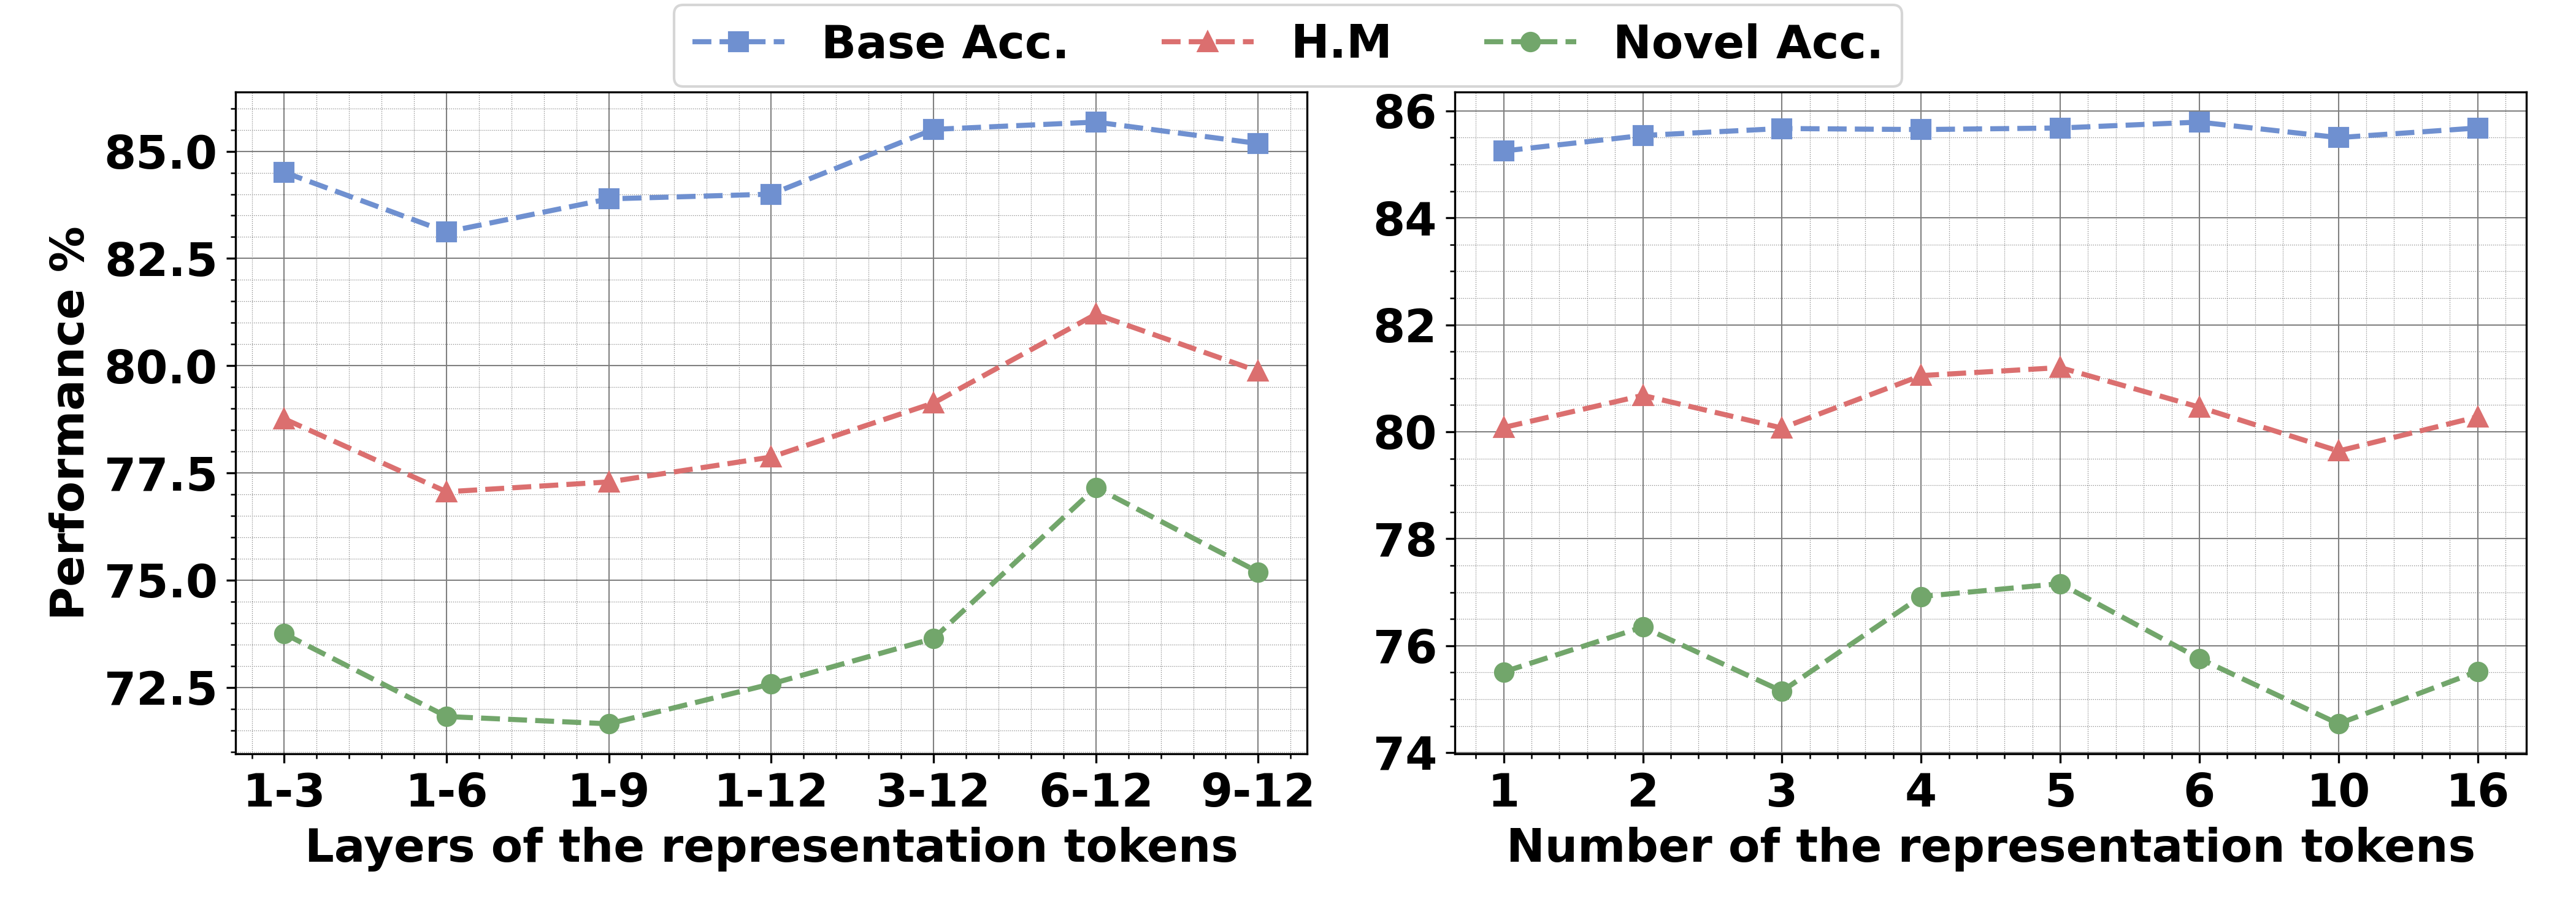
\includegraphics[width=1.0\linewidth]{fig/ablation_layer_N.png}
  \caption{Ablation on layers (left) and $K$ (right).}
  \label{ablation_layers_numbers}
\vspace{-0.5cm}
\end{figure}
%-------------------------------------------------------------------------


%-------------------------------------------------------------------------
\begin{table}[pb]
\centering
\vspace{-0.4cm}
\setlength{\abovecaptionskip}{0.15cm}  
\caption{Ablation on variants (left) and $d_r$ (right).}
\label{ablation_variants_dr}
    \begin{subtable}{0.495\linewidth}
    % \caption{Ablation on Variants\label{ablation_variants}}
    \centering
    \resizebox{0.95\textwidth}{!}{
        \footnotesize
        \begin{tabular}{@{}c|ccc@{}}
        \toprule
        Variants              & Base           & Novel          & HM             \\ \midrule
        w/o L                 & 85.05          & 75.65          & 80.08          \\
        w/o V                 & 82.83          & 75.03          & 78.74          \\
        w/o $\text{DS}_1$     & 83.59          & 77.16          & 80.25          \\
        w/o $\text{DS}_2$     & 85.68          & 73.80          & 79.30          \\
        w/o RS                & \textbf{85.79} & 75.55          & 80.34          \\
        $\text{MMRL}^\dagger$ & 85.60          & 76.02          & 80.55          \\
        \rowcolor[HTML]{EFEFEF} 
        MMRL                  & 85.68          & \textbf{77.16} & \textbf{81.20} \\ \bottomrule
        \end{tabular}
        }
    \end{subtable}
    \begin{subtable}{0.495\linewidth}
    % \caption{Ablation on $d_r$ Settings}
    \centering
    \resizebox{0.965\textwidth}{!}{
        \footnotesize
        \begin{tabular}{@{}c|ccc@{}}
        \toprule
        $d_r$ & Base           & Novel          & HM             \\ \midrule
        32    & 85.27          & 76.85          & 80.84          \\
        128   & 85.42          & 76.74          & 80.85          \\
        256   & 85.63          & 76.84          & 81.00          \\
        \rowcolor[HTML]{EFEFEF} 
        512   & \textbf{85.68} & \textbf{77.16} & \textbf{81.20} \\
        1024  & 85.57          & 76.97          & 81.04          \\
        2048  & 85.53          & 76.91          & 81.00          \\ \bottomrule
        \end{tabular}
        }
    \end{subtable}

\end{table}
%-------------------------------------------------------------------------



\subsection{Ablation Analysis}
All ablation experiments are conducted on base-to-novel generalization across 11 datasets, with results averaged, except for the analysis of $\lambda$ on ImageNet; please refer to the \textbf{Supplementary Material} for the complete $\lambda$ analysis across all datasets.

\noindent \textbf{Variants of MMRL:} The performance of MMRL variants, as shown in \cref{ablation_variants_dr} (left), highlights the contributions of different components. In the variants `w/o L' and `w/o V', where only a single modality of representation tokens is utilized, we observe a performance decline, especially in `w/o V', emphasizing the significance of multimodal interaction and representation features in MMRL. The `w/o $\text{DS}_1$' variant, which omits the Decoupling Strategy and relies only on class features, degrades significantly on base classes, underscoring the role of representation features in capturing downstream knowledge. The `w/o $\text{DS}_2$' variant, using both features for novel class evaluation, also drops notably, suggesting that the representation tokens primarily capture base class features, making transfer to new tasks challenging. The `w/o RS' variant, which excludes the Representation Space, independently initializes textual and visual tokens without multimodal learning. This unimodal approach, while improving base class performance, severely limits generalization to novel classes, indicating the necessity of multimodal learning for effective generalization. Finally, $\text{MMRL}^\dagger$ adopts a biased multimodal learning scheme similar to MaPLe \cite{maple}, where text-side tokens are initialized randomly and mapped to the visual side. Results indicate that this biased approach underperforms compared to MMRL's balanced multimodal learning framework.

\noindent \textbf{Dimension of Representation Space, $d_r$:} As shown in \cref{ablation_variants_dr} (right), adjusting $d_r$ reveals that performance initially increases, followed by a decline as $d_r$ continues to grow. This decline likely stems from overfitting caused by an overly complex representation space.

\noindent \textbf{Layer for Representation Token Insertion:} As depicted in \cref{ablation_layers_numbers} (left), model performance declines when representation tokens are introduced at lower encoder layers. This trend aligns with MMRL's design, as higher layers capture dataset-specific, discriminative features, while lower layers retain generalizable features. Furthermore, MMRL performs poorly on base classes when representation tokens are inserted into lower layers, suggesting that lower-layer features are less adaptable. Performance improves with insertion at higher layers but declines when placed too high, likely due to the reduced number of learnable parameters and limited capacity to influence CLIP's critical parameters.


\begin{table}[t]
\centering
\setlength{\abovecaptionskip}{0.15cm}  
\caption{Ablation on $\alpha$ (left) across 11 datasets and $\lambda$ (right) on ImageNet.}
\label{ablation_alpha_lambda}
    \begin{subtable}{0.46\linewidth}
    % \caption{Ablation on Variants\label{ablation_variants}}
    \centering
    \resizebox{0.9\textwidth}{!}{
        \footnotesize
        \begin{tabular}{@{}c|ccc@{}}
        \toprule
        $\alpha$ & Base           & Novel          & HM             \\ \midrule
        0.0      & 82.96          & 72.34          & 77.29          \\
        0.3      & 84.57          & 75.45          & 79.75          \\
        0.5      & 85.42          & 76.11          & 80.50          \\
        \rowcolor[HTML]{EFEFEF} 
        0.7      & \textbf{85.68} & \textbf{77.16} & \textbf{81.20} \\
        1.0      & 83.79          & 75.49          & 79.42          \\ \bottomrule
        \end{tabular}
        }
    \end{subtable}
    \begin{subtable}{0.46\linewidth}
    % \caption{Ablation on $d_r$ Settings}
    \centering
    \resizebox{0.9\textwidth}{!}{
        \footnotesize
        \begin{tabular}{@{}c|ccc@{}}
        \toprule
        $\lambda$ & Base           & Novel          & HM             \\ \midrule
        0.0       & 77.73          & 70.63          & 73.96          \\
        0.2       & 77.83          & 71.23          & 74.38          \\
        \rowcolor[HTML]{EFEFEF} 
        0.5       & \textbf{77.90} & \textbf{71.30} & \textbf{74.45} \\
        2.0       & \textbf{77.90} & 70.93          & 74.25          \\
        4.0       & 77.67          & 70.73          & 74.04          \\ \bottomrule
        \end{tabular}
        }
    \end{subtable}
\vspace{-0.4cm}
\end{table}


\noindent \textbf{Number of Representation Tokens, $K$:} In \cref{ablation_layers_numbers} (right), increasing $K$ slightly enhances base class accuracy due to additional learnable parameters. For novel classes, accuracy initially improves with $K$ but eventually declines, indicating that an excessive number of tokens may lead to overfitting, reducing generalization capacity.


\noindent \textbf{Balance Weight, $\alpha$:} The parameter $\alpha$ modulates reliance on representation token features versus class token features. Lower $\alpha$ values increase dependence on representation features, heightening overfitting risk due to the learnable projection layer, while higher values shift dependence to class token features, diminishing transferability. As shown in \cref{ablation_alpha_lambda} (left), the optimal $\alpha$ is 0.7.

\noindent \textbf{Penalty Coefficient, $\lambda$:}  The penalty coefficient $\lambda$ regulates the regularization strength by aligning class token features with frozen CLIP’s features. Higher $\lambda$ generally enhances generalization but may restrict transfer flexibility. In \cref{ablation_alpha_lambda} (right), the optimal $\lambda$ for ImageNet is 0.5.


